% =====================================================================
%  precisionMLPs -- lab findings deck (audience: PI + labmates)
%  Compile on Overleaf with XeLaTeX or LuaLaTeX (best fonts);
%  pdfLaTeX also works. Falls back to a clean default theme if the
%  Metropolis theme is unavailable -- figure annotations are anchored
%  in image coordinates, so they render identically either way.
% =====================================================================
\documentclass[aspectratio=169,10pt]{beamer}

\IfFileExists{beamerthemem.sty}{%
  \usetheme{metropolis}
  \metroset{block=fill, sectionpage=none, numbering=fraction}
}{%
  \usetheme{default}
  \usecolortheme{seahorse}
  \setbeamertemplate{navigation symbols}{}
}

\usepackage{graphicx}
\usepackage{booktabs}
\usepackage{amsmath,amssymb}
\usepackage{tikz}
\usetikzlibrary{positioning,calc,arrows.meta}
\usepackage{xcolor}

\graphicspath{{slides_resources/}}

\definecolor{accent}{HTML}{1F6F8B}
\definecolor{hl}{HTML}{E03A1C}
\definecolor{good}{HTML}{2E7D32}
\setbeamercolor{frametitle}{bg=accent}
\setbeamercolor{title separator}{fg=accent}
\setbeamercolor{progress bar}{fg=accent}

% ---------------------------------------------------------------------
%  Helper macros
% ---------------------------------------------------------------------
\newcommand{\bigfig}[2][0.78\textheight]{%
  \centering\includegraphics[height=#1,width=\textwidth,keepaspectratio]{#2}}

% Annotated figure: include #2 (opt #1 = width), draw #3 in NORMALISED
% image coords (x,y in [0,1], origin bottom-left).
\newcommand{\figannot}[3][\textwidth]{%
  \centering
  \begin{tikzpicture}
    \node[anchor=south west,inner sep=0] (IMG) at (0,0)
      {\includegraphics[width=#1,height=0.74\textheight,keepaspectratio]{#2}};
    \begin{scope}[x={(IMG.south east)},y={(IMG.north west)}]
      #3
    \end{scope}
  \end{tikzpicture}}

\newcommand{\look}[1]{\vspace{0.25em}\par
  {\footnotesize\textbf{\color{accent}Read:}~#1}}

\newcommand{\hlcirc}[3]{\draw[hl,very thick] (#1,#2) ellipse [x radius=#3, y radius=#3];}
\newcommand{\hlell}[4]{\draw[hl,very thick] (#1,#2) ellipse [x radius=#3, y radius=#4];}
\newcommand{\hllabel}[3]{\node[hl,font=\footnotesize\bfseries,align=center] at (#1,#2) {#3};}

% ---------------------------------------------------------------------
%  L1-ball (cross-polytope) concept figure -- weight uniformity.
%  +X,+Y toward viewer, +Z up; front (+,+,+) face highlighted.
%  Two-step overlay: init point -> arrow to uniform face-centre.
% ---------------------------------------------------------------------
\newcommand{\Ldiamond}{%
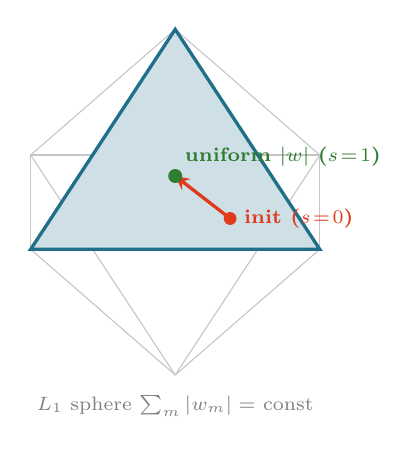
\begin{tikzpicture}[scale=1.05,
    x={(0.92cm,-0.30cm)}, y={(-0.92cm,-0.30cm)}, z={(0cm,1.10cm)},
    >=stealth, line cap=round]
  \def\r{1.9}
  \coordinate (Xp) at (\r,0,0); \coordinate (Xm) at (-\r,0,0);
  \coordinate (Yp) at (0,\r,0); \coordinate (Ym) at (0,-\r,0);
  \coordinate (Zp) at (0,0,\r); \coordinate (Zm) at (0,0,-\r);
  % all edges (light)
  \foreach \a in {Xp,Xm,Yp,Ym}{
    \draw[gray!45,thin] (Zp)--(\a); \draw[gray!45,thin] (Zm)--(\a);}
  \draw[gray!45,thin] (Xp)--(Yp)--(Xm)--(Ym)--cycle;
  % highlighted front face (+,+,+) = one orthant of equal-magnitude weights
  \fill[accent!22] (Xp)--(Yp)--(Zp)--cycle;
  \draw[accent,very thick] (Xp)--(Yp)--(Zp)--cycle;
  % uniform centre (face centroid) and a Xavier-init point on the face
  \coordinate (C) at (0.333*\r,0.333*\r,0.333*\r);
  \coordinate (P) at (0.62*\r,0.24*\r,0.14*\r);
  \onslide<1->{\fill[hl] (P) circle (2.2pt);
    \node[hl,font=\scriptsize\bfseries,anchor=west] at (P) {\,init ($s\!=\!0$)};}
  \onslide<2->{\draw[hl,very thick,->] (P)--(C);
    \fill[good] (C) circle (2.4pt);
    \node[good,font=\scriptsize\bfseries,anchor=south west] at (C) {uniform $|w|$ ($s\!=\!1$)};}
  % axis hint
  \node[gray,font=\scriptsize] at (0,0,-1.18*\r) {$L_1$ sphere $\sum_m|w_m|=$ const};
\end{tikzpicture}}

% ---------------------------------------------------------------------
%  Per-section corner tag: "A . short desc" in the top-right of every
%  content frame. Set once per section with \settag{...}; persists until
%  changed. Empty tag draws nothing (title/section/Overview frames).
% ---------------------------------------------------------------------
\newcommand{\slidetag}{}
\newcommand{\settag}[1]{\renewcommand{\slidetag}{#1}}
% tag sits inside the top banner, right-aligned, in white
\addtobeamertemplate{frametitle}{}{%
  \begin{tikzpicture}[remember picture,overlay]
    \node[anchor=north east,text=white,font=\scriptsize\bfseries,inner sep=0pt]
      at ([shift={(-0.4cm,-0.42cm)}]current page.north east){\slidetag};
  \end{tikzpicture}%
}

% Dedicated section-divider frame: short name + one-line "thing".
\newcommand{\sectiondivider}[2]{%
  {\setbeamercolor{background canvas}{bg=accent}%
   \setbeamercolor{normal text}{fg=white}\usebeamercolor[fg]{normal text}%
   \begin{frame}[plain]
     \centering\vfill
     {\Huge\bfseries #1}\\[0.6em]
     {\color{white}\rule{2.5em}{2pt}}\\[0.7em]
     {\large #2}
     \vfill
   \end{frame}}}

% =====================================================================
\title{Geometry and Optimization of Machine Epsilon MLPs}
\author{Sam Layton}
\date{\today}

\begin{document}

\maketitle
\settag{}

% =====================================================================
\begin{frame}{Overview}
  \small
  \begin{enumerate}
    \item Tested and recreated the exact QI construction
    \item Forget the convolution: just \alert{lstsq the $\Phi$ readout}. It
          works, and is empirically \emph{better}. Some empirical justifications for it:
          (better performance / coefficient closeness / min-norm).
    \item Given the geometry, lstsq \alert{scales and is robust} (input \&
          output noise, width, data).
    \item[$\Rightarrow$] \textbf{So it is solved from $\mathbb{R} \rightarrow \mathbb{R}^n$ for a single hidden layer MLP, using the QI geometry.}
    \item Where might an optimizer fail in finding this geometry? QI geometry has these \alert{three properties}: even centers + halo, $\gamma=O(N)$, uniform weights.
    \item Fourth barrier: Adam can't even do lstsq on a frozen ideal geometry.
    \item How can we assist optimizer in getting to these solutions
    \item Found a plausible construction for 2D: but needs more theory + better testing.
  \end{enumerate}
\end{frame}

% =====================================================================
\section{A.\, The readout is solved}
\settag{A \,$\cdot$\, the readout}
\sectiondivider{A.\ The readout is solved}{Recreate the construction, then solve the readout by least squares.}
% =====================================================================
\begin{frame}{Testing the construction}
  \begin{columns}[T]
    \begin{column}{0.5\textwidth}
      The QI cardinal construction is exact in theory; the only question was
      whether it survives finite precision.
      \begin{itemize}\footnotesize
        \item Extended-precision (mpmath) path: $L_\infty\sim 3\times10^{-15}$
              (machine $\varepsilon$).
        \item \texttt{fp64} path stalls at $\sim\!10^{-12}$ (cancellation in the
              alternating-sign cardinal coefficients $c_j$).
      \end{itemize}
      \vspace{0.3em}
      Baseline established. Do we even need the convolution machinery?
    \end{column}
    \begin{column}{0.5\textwidth}
      \figannot[\textwidth]{qi_floor.png}{%
        
      }
      \look{mpmath (orange) $\to\sim\!10^{-15}$; \texttt{fp64} (blue) floors
        at $\sim\!10^{-12}$.}
    \end{column}
  \end{columns}
\end{frame}

% =====================================================================
\begin{frame}{lstsq $\Phi$ readout $>$ toeplitz solution convolution}
  \begin{columns}[T]
    \begin{column}{0.62\textwidth}
      \bigfig[0.80\textheight]{A02_lstsq.png}
    \end{column}
    \begin{column}{0.38\textwidth}
      Fix the geometry, build $\Phi_{im}=\tanh(\gamma(x_i-c_m))$, and solve the
      readout by least squares.
      \begin{itemize}\footnotesize
        \item lstsq $\le$ QI in \emph{all 48} cells.
        \item In \texttt{fp64}: lstsq flat at $\sim\!10^{-13}$ while the QI
              formula degrades to $\sim\!10^{-10}$ (it inherits the $c_j$
              cancellation).
        \item The Toeplitz machinery is unnecessary once geometry is fixed.
      \end{itemize}
      \look{solid (lstsq) sits at/below dashed (QI) everywhere.}
    \end{column}
  \end{columns}
\end{frame}

% =====================================================================
\begin{frame}{More justifications for lstsq}
  \begin{columns}[T]
    \begin{column}{0.58\textwidth}
      \figannot[\textwidth]{A03_nullspace.png}{%
      }
    \end{column}
    \begin{column}{0.42\textwidth}
      Do QI and lstsq pick the same coefficients for the final layer? In raw space: no. In the row space of $A=[\Phi,\mathbf 1]$: yes. 
      \begin{itemize}\footnotesize
        \item \textbf{Coordinate space:} Large disagreement by $O(1-100)$ (solid-lines). But this disagreement is in the null space of $A$.
        \item \textbf{Row space} (data-visible): coefficients agree with relative percent error $10^{-4}$--$10^{-3}$ (dashed-lines).
        \item lstsq returns the \alert{min-norm} representative of nearly the same solution.
      \end{itemize}
      \look{the vertical gap between solid (full) and dashed (row) \emph{is} the null-space freedom.}
    \end{column}
  \end{columns}
\end{frame}

% =====================================================================

\begin{frame}{Two interesting findings before we go further}
  \begin{columns}[T]
    \begin{column}{0.5\textwidth}
      \centering\textbf{Aside: activation $\Rightarrow$ rank$(A$)}\\[2pt]
      \bigfig[0.6\textheight]{A04_activation.png}
      \par{\footnotesize $\tanh$: null space \emph{constant} ($\dim\approx150$,
      rank $\approx N$) $\Rightarrow$ reaches the floor. GELU: null space
      \emph{grows linearly} in $N$ $\Rightarrow$ 1--3 orders worse, at equal
      conditioning.}
    \end{column}
    \begin{column}{0.5\textwidth}
      \centering\textbf{Rule-out: no weight blowup}\\[2pt]
      \bigfig[0.6\textheight]{A05_blowup.png}
      \par{\footnotesize Readout norm \emph{decreases} with $N$ (power law).
      The $10^{6}$--$10^{7}$ norms at small $N$ are resolution failures, not an optimizer pathology. QI carries only $\sim\!1.25\times$ the min-norm
      vector.}
    \end{column}
  \end{columns}
\end{frame}

% =====================================================================
\begin{frame}{Open questions: A}
  \begin{itemize}
    \item \textbf{Activation null-space regimes: bounded vs growing.} $\tanh$ has
          a bounded (roughly constant) null space (rank $\approx N$) and reaches
          the floor; GELU has an $O(N)$ growing null space (rank $\approx 0.4N$)
          and stalls 1--3 orders short, at comparable conditioning, so it is
          rank, not conditioning, that separates them. \emph{Why?} What property
          of an activation sets the bounded-vs-growing regime: do the kernel
          conditions K1--K4 on $K=\psi^{(r)}$ predict it? Is a bounded null space
          necessary to reach the floor? Map other valid-kernel activations (sin,
          sech, softplus) onto the two regimes.
  \end{itemize}
\end{frame}

% =====================================================================
\section{B.\, Scales and robust to noise}
\settag{B \,$\cdot$\, scaling \& noise}
\sectiondivider{B.\ Scales and robust}{Fixed geometry + lstsq scales with width and data, and tolerates noise.}
% =====================================================================
\begin{frame}{Scales with width and data to the \texttt{fp64} floor}
  \begin{columns}[T]
    \begin{column}{0.64\textwidth}
      \bigfig[0.80\textheight]{B02_scaling.png}
    \end{column}
    \begin{column}{0.36\textwidth}
      Fixed geometry + lstsq, clean data:
      \begin{itemize}\footnotesize
        \item Power-law descent in width until the common floor
              ($\sim\!5\times10^{-14}$).
        \item Activation \& target set the \emph{slope/intercept}, not the
              floor: $\tanh$/GELU steep; ReLU a clean slow $\sim\!N^{-2}$.
        \item Data scaling collapses to the floor past the $W\!+\!1$ threshold.
      \end{itemize}
      \look{top two rows ($\tanh$, GELU) hit the floor; ReLU (bottom) is still
        sliding.}
    \end{column}
  \end{columns}
\end{frame}

% =====================================================================
\begin{frame}{Robust to noise}
  \begin{columns}[T]
    \begin{column}{0.43\textwidth}
      Two separate things.
      \begin{itemize}\footnotesize
        \item \textbf{Sample positions ($x$):} random and uniform samples both
              stay at the floor. Precision is set by center placement, not by
              where you sample.
        \item \textbf{Centers:} random centers (green, red) plateau 2--3 orders
              above and never recover.
        \item \textbf{Output noise ($y$):} a hard floor near the noise level;
              adding data recovers it only at the $1/\sqrt{n}$ rate. Reaching
              $\varepsilon$ from $10^{-2}$ noise would need $\sim\!10^{23}$
              samples.
      \end{itemize}
    \end{column}
    \begin{column}{0.57\textwidth}
      \centering
      {\scriptsize\textbf{Sample positions vs.\ centers}}\\[1pt]
      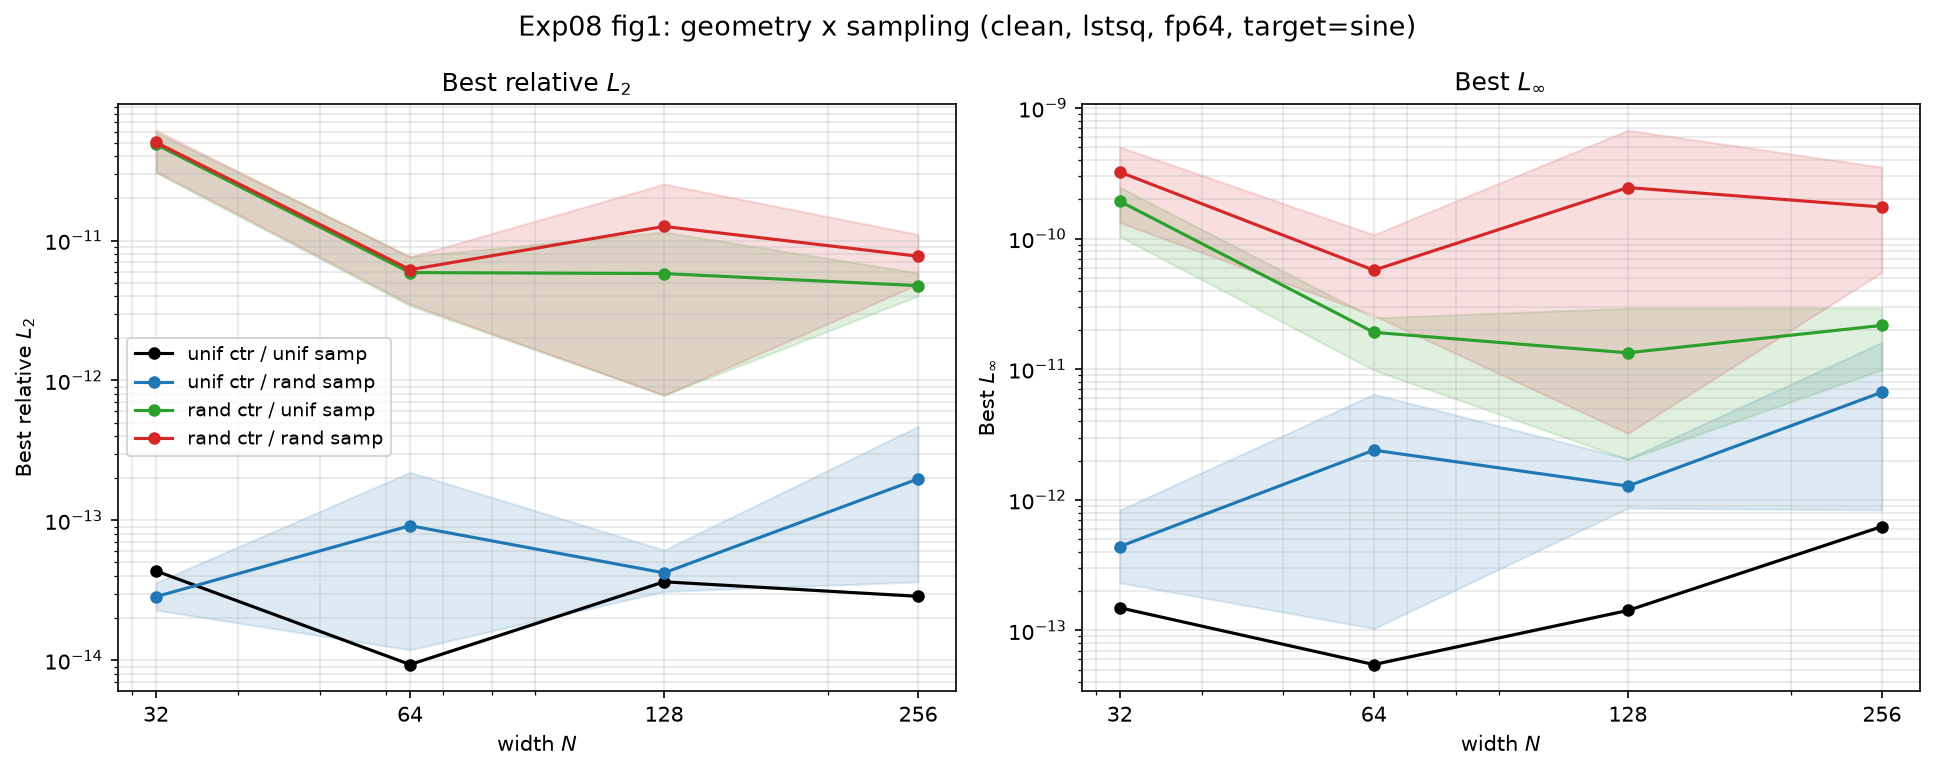
\includegraphics[width=\textwidth,height=0.32\textheight,keepaspectratio]{B01_geometry.png}\\[4pt]
      {\scriptsize\textbf{Output noise + more data}}\\[1pt]
      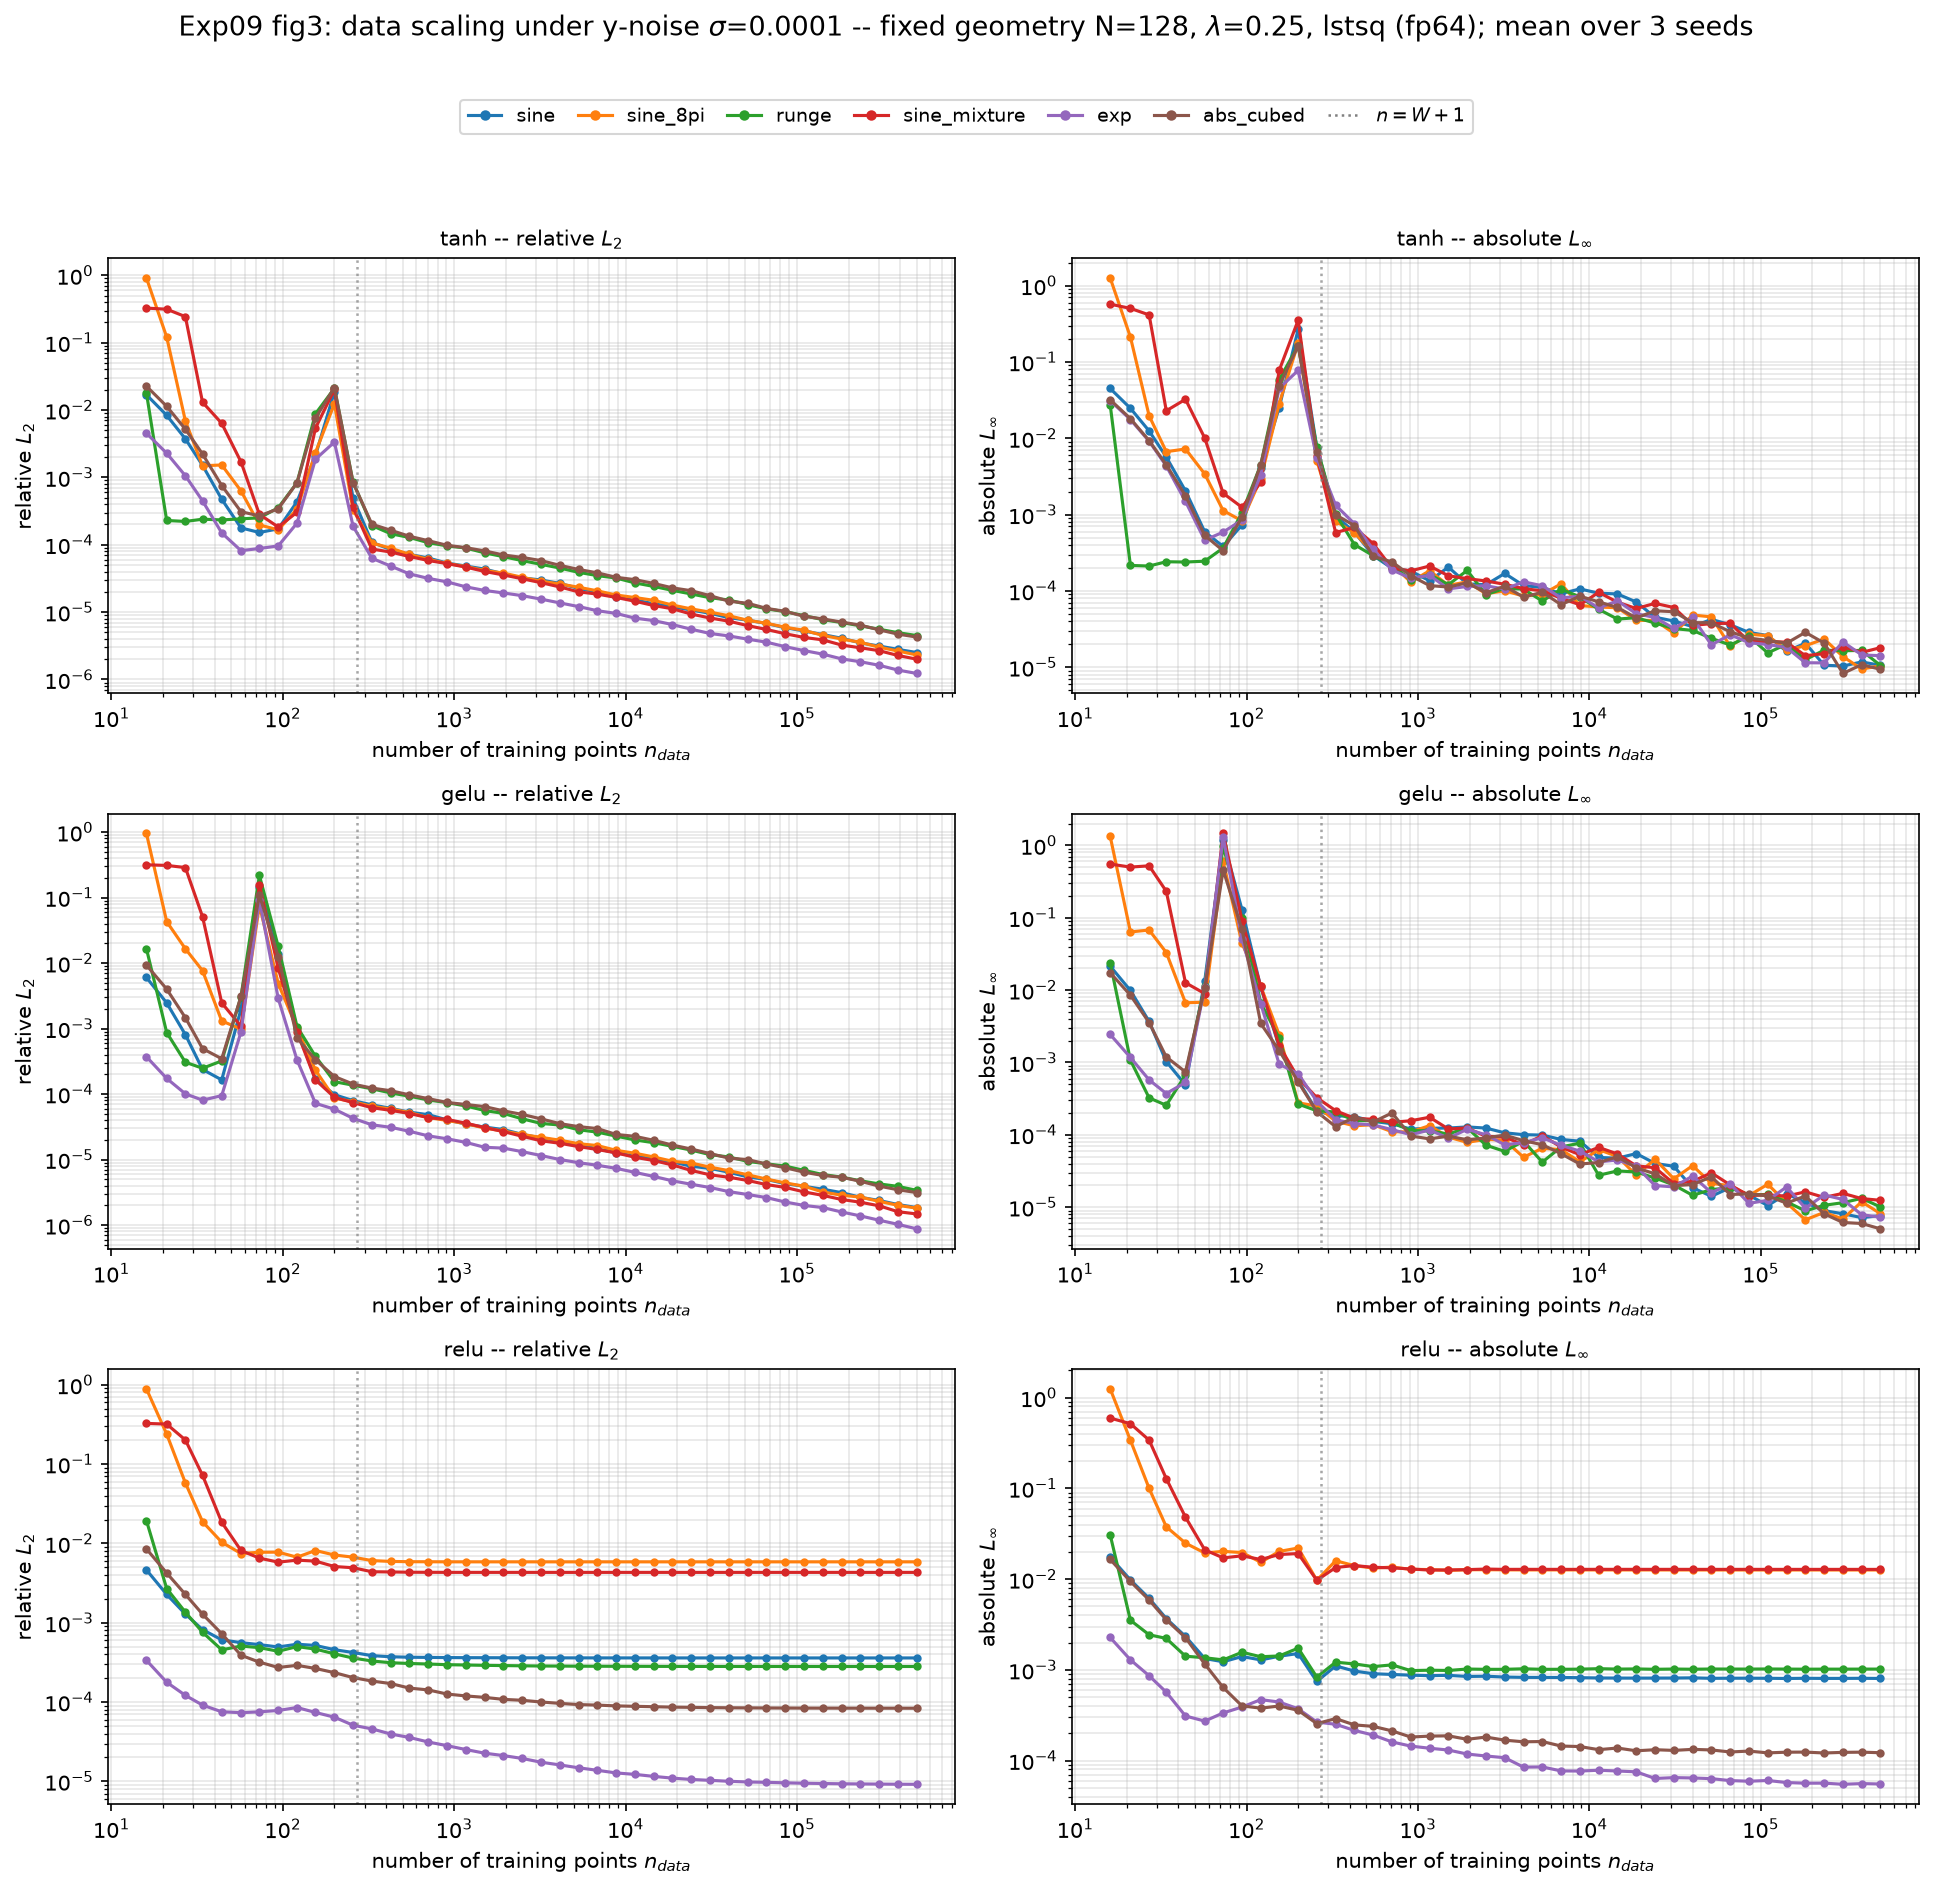
\includegraphics[width=\textwidth,height=0.40\textheight,keepaspectratio]{B02_datanoise.png}
    \end{column}
  \end{columns}
\end{frame}

% =====================================================================
\begin{frame}[c]{So $\mathbb{R}\rightarrow\mathbb{R}^n$ is solved with the same geometry}
  \begin{center}
  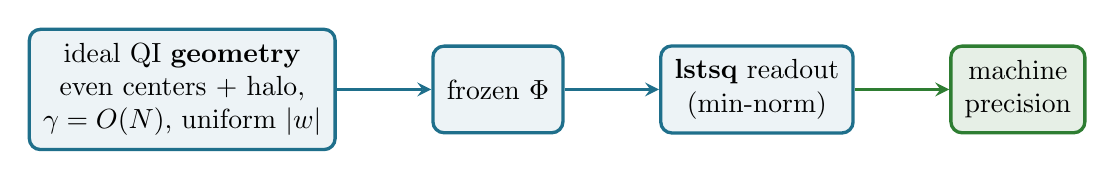
\begin{tikzpicture}[node distance=8mm,>=stealth,
      box/.style={draw=accent,very thick,rounded corners,fill=accent!8,
                  align=center,minimum height=11mm,inner sep=5pt}]
    \node[box] (g) {ideal QI \textbf{geometry}\\even centers + halo,\\$\gamma=O(N)$, uniform $|w|$};
    \node[box,right=12mm of g] (p) {frozen $\Phi$};
    \node[box,right=12mm of p] (r) {\textbf{lstsq} readout\\(min-norm)};
    \node[box,right=12mm of r,fill=good!12,draw=good] (e) {machine\\precision};
    \draw[->,very thick,accent] (g)--(p);
    \draw[->,very thick,accent] (p)--(r);
    \draw[->,very thick,good] (r)--(e);
  \end{tikzpicture}
  \end{center}
  \vspace{0.4em}
  The readout is a convex least-squares solve, and it is robust. All the remaining difficulty is in producing the geometry with an optimizer.\\
  \vspace{1em}
  But why would we care about an optimizer that can find the geometry. The hypothesis is this: \textbf{If an optimizer can find the machine epsilon solution for $\mathbb{R}\rightarrow\mathbb{R}^n$ problems, it might be able to solve multilayer $\mathbb{R}^m\rightarrow\mathbb{R}^n$ problems.}
\end{frame}

% =====================================================================
\section{C.\, Probing the QI geometry}
\settag{C \,$\cdot$\, the geometry}
\sectiondivider{C.\ Probing the QI geometry}{What must the first-layer geometry satisfy to hit machine precision?}
% =====================================================================
\begin{frame}{Three properties of the ideal geometry}
  We localize precision to three first-layer conditions. Training violates all
  three.
  \begin{enumerate}\small
    \item \textbf{Bandwidth:} $\gamma=O(N)$, i.e.\ $\lambda=\gamma h\approx0.25$
          fixed. Adam/Xavier sit at $\gamma=O(1)$, so $\lambda\to0$ as width
          grows.
    \item \textbf{Centers:} a uniform grid over $[-1,1]$, \emph{plus a halo} of
          extra nodes outside the domain (boundary stabilization).
    \item \textbf{Weights:} uniform magnitude: the weight vector sits at the
          \emph{center of a face} of the $L_1$ sphere $\sum_m|w_m|=$ const
          (sign pattern is shown to be free).
  \end{enumerate}
  \vspace{0.4em}
  {\footnotesize The next slides sweep each condition off its ideal value and
  watch precision fail.}
\end{frame}

% =====================================================================
\begin{frame}{Property 1: bandwidth $\gamma=O(N)\approx N/8$ is the dominant knob}
  \begin{columns}[T]
    \begin{column}{0.6\textwidth}
      \bigfig[0.80\textheight]{C01_tradeoff.png}
    \end{column}
    \begin{column}{0.4\textwidth}
      \begin{itemize}\footnotesize
        \item Error vs.\ $\lambda=\gamma h$ is U-shaped: ill-conditioning on the
              left, aliasing and cancellation on the right.
        \item Optimal $\lambda^\star\!\approx\!0.25$, flat across width and across
              frequency (also tested on $\sin(2\pi k x)$, $k$ up to 16). Set
              $\gamma\approx N/8$: scale with $N$, not $W$.
        \item lstsq's basin is wide, QI's is pinned. Worth $\sim\!8$--$10$ orders.
        \item Trained nets instead drive $\lambda\to0$ as width grows.
      \end{itemize}
    \end{column}
  \end{columns}
\end{frame}

% =====================================================================
\begin{frame}{Bandwidth basin: $\lambda^\star$ is flat in width}
  \begin{columns}[T]
    \begin{column}{0.62\textwidth}
      \bigfig[0.80\textheight]{C03_basin.png}
    \end{column}
    \begin{column}{0.38\textwidth}
      On the ideal uniform geometry, sweep $\lambda$ and read off the basin
      (green line = center $\lambda^\star$, band = its range, dashed = $0.25$).
      \begin{itemize}\footnotesize
        \item The basin is wide; $\lambda^\star$ stays near $0.2$--$0.27$ as $N$
              (and $W$) grow.
        \item So $\gamma^\star=\lambda^\star N/2\approx N/8$, across targets and
              widths.
        \item This is the magnitude the inner weights should take.
      \end{itemize}
    \end{column}
  \end{columns}
\end{frame}

% =====================================================================
\begin{frame}{A second near-floor mode at large $N$}
  \begin{columns}[T]
    \begin{column}{0.66\textwidth}
      \figannot[\textwidth]{C03_basingrid.png}{%
        \hlell{0.875}{0.575}{0.05}{0.05}
        \hllabel{0.875}{0.665}{second dip};
      }
    \end{column}
    \begin{column}{0.34\textwidth}
      Each panel: error vs $\lambda$ for one target (row) and width (column).
      \begin{itemize}\footnotesize
        \item At large $N$ a second near-floor region appears at small
              $\lambda\!\approx\!0.05$.
        \item For runge it slightly beats $\lambda=0.25$.
        \item Open: aliasing artifact, or a usable small-bandwidth regime that
              widens with $N$?
      \end{itemize}
    \end{column}
  \end{columns}
\end{frame}



% =====================================================================
\begin{frame}{Property 2: centers must be uniform (+ halo)}
  \begin{columns}[T]
    \begin{column}{0.56\textwidth}
      \figannot[\textwidth]{C04_centers.png}{%
        \hlell{0.27}{0.17}{0.16}{0.035}
      }
      \par{\footnotesize \emph{Below:} the layouts swept (seed 0).}
      \bigfig[0.30\textheight]{C04_numberline.png}
    \end{column}
    \begin{column}{0.44\textwidth}
      Only the uniform grid reaches machine precision; \alert{every} non-uniform
      placement plateaus 2--3 orders above and never descends with width.
      \begin{itemize}\footnotesize
        \item Controlled $W$, interval span, $\gamma$
        \item Does \emph{not} track $\mathrm{cond}(\Phi)$ ($\sim\!10^{19}$ for
              all): coverage, not conditioning.
        \item ``Trained'' centers concentrate inside $[-1,1]$ but still have some halo.
      \end{itemize}
      \look{black (uniform) rides $\sim\!10^{-14}$; all others sit far above.}
    \end{column}
  \end{columns}
\end{frame}

% =====================================================================
\begin{frame}{Center uniformity is monotone}
  \begin{columns}[T]
    \begin{column}{0.66\textwidth}
      \bigfig[0.80\textheight]{C05_centers_interp.png}
    \end{column}
    \begin{column}{0.34\textwidth}
      Interpolate centers from random ($t\!=\!0$) to the uniform grid
      ($t\!=\!1$), at different gamma levels.
      \begin{itemize}\footnotesize
        \item Correct lambda regime is highest leverage
        \item Right column (error vs center uniformity): every line falls as $t\to1$. More uniform is strictly better, with no intermediate dip.
        \item The largest drop is the final nudge onto the exact grid.
        \item Same behavior across initialization seeds.
        \item Uniformity makes deeper and wider lambda valleys
      \end{itemize}
      \look{in the heatmaps (left), the dark band sits at the right edge
        ($t\!=\!1$) for every width.}
    \end{column}
  \end{columns}
\end{frame}


% =====================================================================

\begin{frame}{Property 3: uniform weights = center of an $L_1$ face}
  \begin{columns}[T]
    \begin{column}{0.5\textwidth}
      \centering
      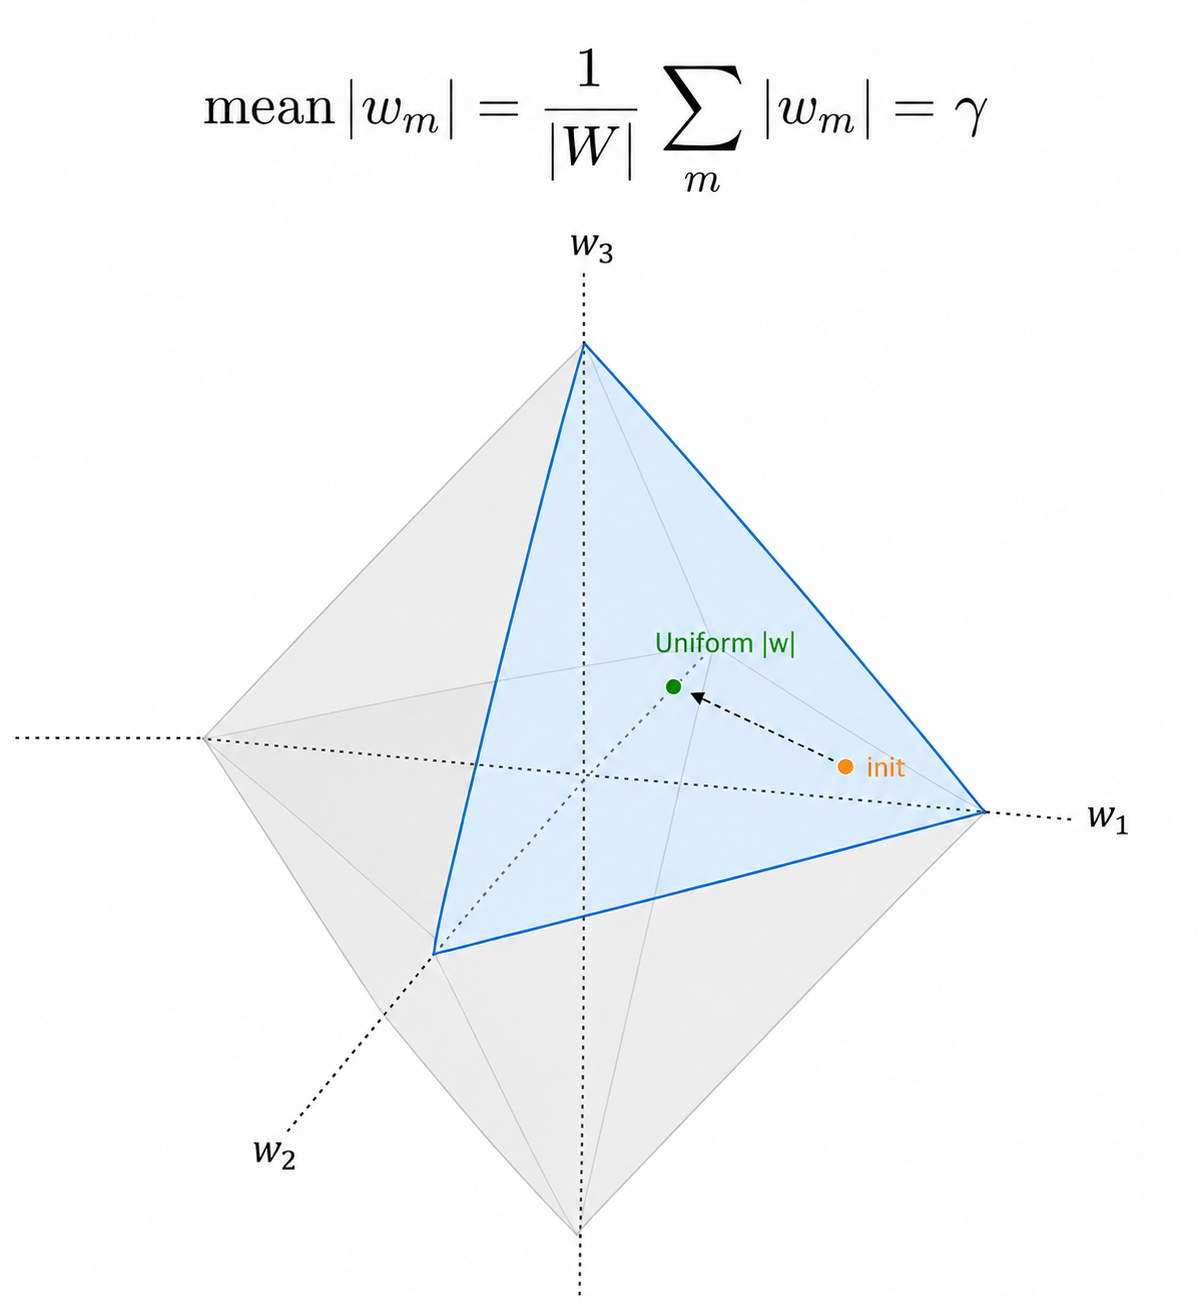
\includegraphics[height=0.66\textheight]{L1_diamond.png}
    \end{column}
    \begin{column}{0.5\textwidth}
      Hold the total weight magnitude $\sum_m|w_m|=\gamma$ fixed (the $L_1$
      sphere, not $L_2$) and interpolate $s$ from a random-magnitude init to the
      \alert{uniform-magnitude face center}.
      \begin{itemize}\footnotesize
        \item In the viable $\lambda$ regime, uniform weights are best: a 2--5
              order win at $N\!=\!128$.
        \item The effect is conditional on $\lambda$, and the path is
              non-monotone (a hump, two slides on).
        \item Sign pattern carries no information: which face you pick does not
              matter.
      \end{itemize}
    \end{column}
  \end{columns}
\end{frame}

% =====================================================================
\begin{frame}{Weight uniformity holds at high frequency ($\sin 8\pi x$)}
  \begin{columns}[T]
    \begin{column}{0.66\textwidth}
      \bigfig[0.80\textheight]{C05_weights_8pi.png}
    \end{column}
    \begin{column}{0.34\textwidth}
      The same weight sweep for a high-frequency target ($\sin 8\pi x$, tanh).
      Rows are widths.
      \begin{itemize}\footnotesize
        \item Heatmaps (left): the dark, near-floor band sits at uniform weights
              in the viable $\lambda$ band.
        \item Middle: the $\lambda$ valley deepens toward uniform weights.
        \item The weight-uniformity win is not specific to low frequency.
      \end{itemize}
    \end{column}
  \end{columns}
\end{frame}

% =====================================================================
\begin{frame}{Interaction: weights and centers couple one way}
  \figannot[\textwidth]{C05_interaction_exp.png}{%
    \draw[accent,very thick] (0.245,0.89) ellipse [x radius=0.013,y radius=0.05];
    \node[accent,font=\scriptsize\bfseries,align=center] at (0.12,0.98){exact QI\\(best)};
    \draw[accent,very thick] (0.245,0.12) ellipse [x radius=0.013,y radius=0.05];
    \draw[accent,very thick,->] (0.40,0.05)--(0.256,0.12);
    \node[accent,font=\scriptsize\bfseries,align=center] at (0.47,0.045){uniform $w$ + random $c$ (worst)};
  }
  \vspace{0.1em}
  {\footnotesize Sweep weight uniformity ($s$) and center uniformity ($t$)
  together (exp target, $N\!=\!64$). \textbf{Centers ($t$): monotone}, always
  helps. \textbf{Weights ($s$): conditional.} Uniform weights pay off only once
  the centers are uniform. Uniform $w$ + random $c$ is the worst corner, below
  the random start: the coupling runs one way, weights need centers, not the
  reverse.}
\end{frame}



% =====================================================================
\begin{frame}{The weight path has a hump: soft neurons explain it}
  \begin{columns}[T]
    \begin{column}{0.62\textwidth}
      \figannot[\textwidth]{C06_softneuron.png}{%
        \hllabel{0.30}{1.05}{protect smallest\\$\Rightarrow$ hump gone};
        \hllabel{0.78}{1.05}{placebo (random)\\$\Rightarrow$ hump stays};
      }
    \end{column}
    \begin{column}{0.38\textwidth}
      Sweeping toward uniform weights, error \emph{rises} mid-path: the loss
      of the \alert{soft (small-$\gamma$) neurons}, whose
      $\tanh(w(x-c))\approx w(x-c)-\tfrac13 w^3(x-c)^3$ span a low-degree
      polynomial basis that cheaply fits smooth targets.
      \begin{itemize}\footnotesize
        \item Protecting them (not a random same-size set) \emph{flattens} the
              hump: causal, $\sim\!250\times$ on $e^x$.
        \item Effect tracks target convexity.
        \item Hints at a deliberate \emph{cascaded multi-band} geometry.
      \end{itemize}
    \end{column}
  \end{columns}
\end{frame}


% =====================================================================
\begin{frame}{Implicating hypothesis: spread out and sharp}
  The precision-admitting geometry has two ingredients at once.
  \begin{itemize}
    \item \textbf{Spread out:} centers cover the domain uniformly, plus a halo. This is the coverage that lets the readout fit every part of the target.
    \item \textbf{Sharp enough:} $\gamma=O(N)$, so each kernel is narrow enough to resolve detail at the grid scale.
  \end{itemize}
  \vspace{0.3em}
  Coverage without sharpness underfits; sharpness without coverage leaves gaps. Both together reach machine precision. But low magnitude weights in the first layer are extra helpful in convex functions. \\
  \vspace{0.3em}
  The hypothesis: any geometry that is simultaneously well spread out and sharp enough resolves the target to the floor, and an optimizer steered toward such a geometry should reach it too. (while a few soft weights do some heavy lifting)
\end{frame}

% =====================================================================
\begin{frame}{Open questions: C}
  \begin{columns}[T]
    \begin{column}{0.5\textwidth}
      \begin{itemize}\footnotesize
        \item \textbf{Precision vs.\ generalization (mask the data).} The
              uniform-$\gamma$ geometry is all one sharp scale, so it may
              extrapolate badly in data-poor regions. Mask parts of the domain
              and compare held-out error: Adam vs.\ cascade + lstsq vs.\ QI. Do
              the cascade's soft bands recover generalization? Check the tradeoff
              when soft weights are frozen.
        \item \textbf{Cascaded multi-band geometry.} Build it by hand: the
              uniform grid at the ideal $\gamma$ plus a smaller evenly-spaced set
              of low-bandwidth (soft) neurons, maybe a couple of intermediate
              bands. Does it beat plain-uniform and the accidental Xavier soft
              tail? How should band count, spacing, and ratios scale with $N$?
        \item \textbf{Soft-neuron protection and residual-fitting.} Is freezing
              the soft neurons better than full uniformity (tentatively yes for
              convex targets)? Is the $\sim\!10\times$ floor gain at $N\!=\!256$
              real or a seed fluke (fades by $512$)? Is multistage fitting just
              ``soft neurons coarse-fit, sharp neurons fit the residual''?
      \end{itemize}
    \end{column}
    \begin{column}{0.5\textwidth}
      \begin{itemize}\footnotesize
        \item \textbf{Curvature-adaptive uniform centers (1D + 2D).} Denser
              spacing in high-curvature regions while staying locally uniform,
              not random clustering. Does it beat the uniform grid, e.g.\ get
              runge to the floor at $N\!=\!32$? In 2D, coverage near the bumps
              instead of uniform over the disk.
        \item \textbf{Second bandwidth mode near $\lambda\!\approx\!0.05$.} At
              large $N$ a second near-floor region appears at small bandwidth
              (runge slightly beats $\lambda=0.25$). Aliasing, or a genuinely
              usable small-bandwidth regime? Does it keep widening with $N$?
        \item \textbf{The last-mile step change.} Why does the final nudge to
              fully uniform weights and centers give a sudden jump in precision,
              not gradual improvement? (low priority)
      \end{itemize}
    \end{column}
  \end{columns}
\end{frame}

% =====================================================================
\section{D.\, Can the optimizer find it?}
\settag{D \,$\cdot$\, optimization}
\sectiondivider{D.\ Can the optimizer find it?}{Gradient descent can't even solve the readout; what does work?}
% =====================================================================
\begin{frame}{The fourth barrier: first-order descent on a frozen ideal geometry}
  \begin{columns}[T]
    \begin{column}{0.58\textwidth}
      \figannot[\textwidth]{D01_stall.png}{%
        \draw[hl,very thick,<->] (0.215,0.115) -- (0.215,0.275);
        \hllabel{0.33}{0.20}{$\sim$10-order\\gap};
      }
    \end{column}
    \begin{column}{0.42\textwidth}
      Easiest possible rung: geometry frozen at the ideal, only the convex
      readout left to fit.
      \begin{itemize}\footnotesize
        \item Adam stalls at $\sim\!10^{-3}$; lstsq on the \emph{identical}
              $\Phi$ reaches $\sim\!10^{-13}$.
        \item Weights stay $O(1)$, so this is not blowup; the failure is
              first-order descent on $\mathrm{cond}(\Phi)\!\sim\!10^{19}$.
      \end{itemize}
      \alert{So even the solved sub-problem defeats gradient descent.} Don't
      descend the readout; solve it.
    \end{column}
  \end{columns}
\end{frame}

% =====================================================================
\begin{frame}{What does work: good init $\to$ train $\to$ final lstsq refit}
  \begin{columns}[T]
    \begin{column}{0.5\textwidth}
      \centering{\footnotesize\textbf{Training regime (QI init)}}\\[1pt]
      \bigfig[0.58\textheight]{D02_training.png}
    \end{column}
    \begin{column}{0.5\textwidth}
      \centering{\footnotesize\textbf{Initialization (frozen) + lstsq}}\\[1pt]
      \bigfig[0.58\textheight]{D02_init.png}
    \end{column}
  \end{columns}
  \vspace{0.2em}
  {\footnotesize Three results (\texttt{fp32}): \textbf{(1)} QI init + train both
  layers beats standard-init by 2--3 orders; \textbf{(2)} QI init + train +
  \alert{final lstsq refit recovers the floor} ($\sim\!5\times10^{-14}$) from the
  \emph{trained} geometry (the geometry survives training); \textbf{(3)}
  scaled-Xavier (right $\gamma$, inexact centers) generalizes the gain, so
  $\gamma=O(N)$ is the transferable lever. Extends to $1\!\to\!\mathbb{R}^m$ via
  shared geometry + per-coordinate lstsq.}
\end{frame}

% =====================================================================
\begin{frame}{Open questions: D}
  \begin{columns}[T]
    \begin{column}{0.5\textwidth}
      \begin{itemize}\footnotesize
        \item \textbf{Reparameterization (expD03).} Does optimizing in natural
              coordinates let plain gradient descent reach the floor that raw
              $(w,b)$ can't? log-$\gamma$; one global $\lambda$; dimensionless
              centers $c_k=-1+h(k+\delta_k)$; scaled readout $\alpha=a\gamma$.
              Each with a final lstsq refit. Direct test of the one-way coupling.
        \item \textbf{What does the trained geometry look like, and did it
              move?} Are a trained net's centers uniform, what is their spread
              and $\gamma$? With QI init, how much do the first-layer params move
              before the refit (and for runge)?
        \item \textbf{Initialization regimes in greater depth.} Expanding on
              expD02: what properties of the trained solutions should we test in
              the init regime? Is there an optimizer + initialization that work
              better? This is the real question.
      \end{itemize}
    \end{column}
    \begin{column}{0.5\textwidth}
      \begin{itemize}\footnotesize
        \item \textbf{Variable projection (expD04).} Solve the readout exactly by
              lstsq at every step; optimize only the nonlinear geometry
              $\theta=(\lambda,\delta_k)$ with Gauss-Newton / LM / quasi-Newton.
              Does it reach the floor where end-to-end Adam stalls?
        \item \textbf{Can any optimizer solve the lstsq readout?} First-order
              Adam can't (the 4th barrier). Can a second-order / quasi-Newton
              method get there: SSBroyden, LM, or a preconditioned solver?
        \item \textbf{Geometry-ladder levels 4--7.} Relax more: fixed $\gamma$ +
              free centers, then free $\gamma$ + free centers, readout solved or
              trained. Pinpoint which relaxation first loses precision.
        \item Seed-average the finer expD02 trends (coverage vs uniformity;
              scaled vs clean init).
      \end{itemize}
    \end{column}
  \end{columns}
\end{frame}

% =====================================================================
\section{E.\, Extending to 2D}
\settag{E \,$\cdot$\, 2D}
\sectiondivider{E.\ Extending to 2D}{Does the fixed-geometry + lstsq recipe carry to 2D?}
% =====================================================================
\begin{frame}{2D: same story, modulo more theory}
  \begin{columns}[T]
    \begin{column}{0.5\textwidth}
      \bigfig[0.58\textheight]{E01_targets.png}
      \par{\footnotesize Four targets on the unit disk.}
    \end{column}
    \begin{column}{0.5\textwidth}
      \bigfig[0.74\textheight]{E01_suite.png}
    \end{column}
  \end{columns}
  \vspace{0.1em}
  {\footnotesize Fixed \emph{Radon-ridge} geometry + lstsq reaches the
  \texttt{fp64} floor ($\sim\!6\times10^{-14}$) on smooth \texttt{gauss\_bump}
  (top row), best/tied on 3 of 4 targets at the largest width. \texttt{runge2d}
  (spike) stays resolution-limited. Placement decides precision, as in 1D, but
  the right ridge construction and $\lambda(N)$ scaling still need to be
  worked out.}
\end{frame}

% =====================================================================
\begin{frame}{Open questions: E}
  \begin{itemize}
    \item \textbf{Curvature-aware 2D coverage.} The 2D half of the merged
          Checkpoint C curvature item: denser-but-locally-uniform coverage near
          the bumps / high-curvature regions instead of uniformly over the disk.
    \item \textbf{Does optimal $\lambda$ drift with $N$ in 2D?} It looks like it
          may decrease slightly as $N$ grows. Confirm or rule out.
    \item \textbf{Do extended precision and larger $N$ push the other smooth 2D
          targets to the floor?} A more robust treatment, as it appears they
          will.
  \end{itemize}
\end{frame}

% =====================================================================
\section{Frontier}
\settag{}
\sectiondivider{Frontier}{Depth, higher dimension, and applications.}
% =====================================================================
\begin{frame}{Frontier: depth, dimension, applications}
  \begin{columns}[T]
    \begin{column}{0.5\textwidth}
      \begin{itemize}\footnotesize
        \item \textbf{1D and 2D real physics task} end-to-end with the
              constructed geometry.
        \item \textbf{Depth.} Stack the construction across layers (delay until
              the one-hidden-layer case is understood and a good optimization /
              init strategy is found). First step: just try the initialization
              on multiple layers.
        \item \textbf{Higher output dim ($\to\mathbb{R}^m$).} Empirical check;
              works in theory. Shared geometry + per-coordinate lstsq is partly
              shown for $1\!\to\!\mathbb{R}^m$; push to more outputs and harder
              targets.
      \end{itemize}
    \end{column}
    \begin{column}{0.5\textwidth}
      \begin{itemize}\footnotesize
        \item \textbf{Higher input dim ($\mathbb{R}^n\!\to$).} The harder open
              part: higher input dimension plus depth (the 2D Radon recipe is
              step 1). Domain matters, since the init works over the relevant
              region.
        \item \textbf{Non-MSE losses.} How does the method behave under
              cross-entropy or other non-MSE objectives?
        \item \textbf{Transformer init.} Initialize a transformer's first hidden
              layers this way (needs depth, higher input dimension, and domain
              solved first).
      \end{itemize}
    \end{column}
  \end{columns}
\end{frame}

% =====================================================================
{
\setbeamercolor{background canvas}{bg=accent}
\setbeamercolor{normal text}{fg=white}
\usebeamercolor[fg]{normal text}
\begin{frame}[plain]
  \vfill
  \begin{center}
    {\Large\bfseries The readout is solved. The geometry is the problem.}\\[0.8em]
    {\large Even on a frozen ideal geometry, gradient descent can't do lstsq,\\
    so the open question is reaching that geometry, not fitting on it.}
  \end{center}
  \vfill
\end{frame}
}

\end{document}